% Planetary Research - A diamond open access journal
%
% Author Submission Template for Latex
% Last modified: July 18, 2026

% Please add a manuscript type and preview option to the
% documentclass command.
%
% Manuscript type:
%     article
%     reviewarticle
%     letter
%     numericalcode
%     dataset
%     missions
%     introduction
%     editorial
%     commentary
% Preview options:
%     review (for submissions)
%     final (for preprints)
\documentclass[article,review]{planetary}


\usepackage{chemformula}
\usepackage{float}
\usepackage{chemformula}
\usepackage{siunitx}



% ------ Title block --------------------------------------------------
% Add a title and short title
\title{The \textit{Catalogue Astrochimique de Sections Efficaces d'Ionisation} (CASEI): A Database Of Low Energy Total Ionisation Cross-Section For Astrochemical Purpose}
\shorttitle{CASEI: A Database Of Low Energy Total Ionisation Cross-Section For Astrochemical Purpose}

% ------ Author block -------------------------------------------------
% Fill in all authors, their ORCID iDs, and affiliations.
% Each author must have an ORCID iD.
\author[1]{Lilian Heydel \orcid{0000-0000-0000-0000}}
\author[1]{David Dubois \orcid{0000-0000-0000-0000}}

\affil[1]{Centre de Recherche sur les Ions, les Matériaux et la Photonique Université Caen Normandie, GANIL, ENSICAEN, CNRS, CEA, Normandie
Univ, CIMAP UMR6252, F-14000 Caen, France., ROR ID}
\affil[2]{Affiliation of Second Author, City, Country, ROR ID}

\setcorrespauth{Heydel Lilian} % Name of the corresponding author
\setcorrespmail{lilian.heydel@ganil.fr} % email of the corresponding author

% ------ BIB file -----------------------------------------------------
\addbibresource{Docu_BDSEI.bib} % replace by the name of your .bib file

% ------ Date ---------------------------------------------------------
\date{} % leave empty

% ------ Document -----------------------------------------------------
\begin{document}
% \nocite{*}

\maketitle
\thispagestyle{firstpage}

\correspondingauthor % print corresponging author

% ------ Submission and Revision Dates --------------------------------
% Please provide the submission date, all revision dates,
% and the acceptance date. Use \today when appropriate.
\submissiondate{1st January 2026}
% \revisiondate{\today}
% \accepteddate{\today}

% ------ Special Issues -----------------------------------------------
% If the manuscript is submitted as part of a special issue, uncomment
% the following command and provide the special issue name.
% \specialissue{Special issue name}

\mstype{\articletype} % print manuscript type

% ------ Word and character counts ------------------------------------
% Provide the character count of the summary
\summarycharactercount{($\le$ 350 characters)}

\IfStrEq{\articletype}{LETTER}{
% For letters, provide the letter word count (abstract + main text
% + captions) and methods word count.
\letterwordcount{($\le$ 4500)}
\methodswordcount{($\le$ 3000 words)
}}{
% For all other manuscript types, provide the abstract word count.
\abstractwordcount{($\le$ 250 words)}
}

\stitle{\insertshorttitle} % print short title

% ------ Summary ------------------------------------------------------
\summary{A short summary that is 350 or fewer characters in length. The summary will appear before the manuscript abstract and will appear in the issue's table of contents. Summaries should in general be written in full sentences, though other formats may be considered when they respect the character limit.}

% ------ Abstract -----------------------------------------
\begin{abstract}
All submissions to Planetary Research must use the official journal template. By using this template, the authors ensure that all metadata required by the journal are provided, that all elements of the manuscript are present, and that the manuscript is formatted according to the journal's standards. The use of the journal template also ensures that the manuscript can be processed as part of the journal's post-acceptance production pipeline. Manuscript submissions that do not follow the journal's submission guidelines will be systematically rejected without review. The abstract must contain 250 words or less, without line breaks. It should provide a clear understanding of the work without requiring the reader to consult the entire article. The abstract must be self-contained: it should not include references, and any abbreviations or acronyms must be introduced. The abstract should provide the context or background for the study and state the basic procedures, main findings and conclusions.
\end{abstract}

% ------ License ------------------------------------------------------
% If you intend to distribute this manuscript, consider adding a
% CC-BY license by uncommenting the following line
\license{}

\newpage

\section{Methodology}

The methodology employed in this work is based around the 3-dimensionnal geometry of each molecules.

\subsection{Molecular geometry pipeline}
One of the most extensive database for chemical species is PubChem \parencites{kimPubChem2025Update2025}. Practically all of the molecular species present in the database have 3D conformers available to download. The files associated to those conformers, \verb|.xyz| files, consits in the space position of each atom in 3D space. The code employed in this work make a request at PubChem server with the name of the searched molecule and fetch for the 3D structure as for other properties such as the formula. The 3D conformer catalogue of Pubchem was, as their documentation suggests\footnote{\url{https://pubchem.ncbi.nlm.nih.gov/docs/pubchem3d}}, calculated using advanced quantum computational methods of atomic-force fields repultation, with the assurance of a great accuracy between experimental, theoritical and modeled 3D conformers (see \cite{boltonPubChem3DConformerGeneration2011}). In this case, atomic coordinates should already be optimized and no further optimization is needed (see appendix \ref{app:geom}).



One problem emerge regarding molecules with no 3D conformer available. While they represent a very small fraction of this database, and appears as \textit{niche} astrochemically speaking at first glance, they do represents molecules with a certain degre of interest. For instance, Germane \ch{GeH4} could be present in the atmosphere of giant planets \parencites{coriceHypotheticalChemicalSpectroscopic1972,mosesAtmosphericChemistryUranus2020} as well as arsenic bearing molecules \parencites{bezardDetectionArsineSaturn1989,roedererDETECTIONELEMENTSALL2012}. First calculations were initally made using 2D structure (\textit{e.g} with $x$ and $y$ positions and $z$ as vector fullfilled with zeroes), but it was quickly proven to be a  wrong approach. While it could be possible to get 3D conformers from other sources (like Jmol ;\parencites{hansonJmolParadigmShift2010}), it is easier for automated workflow to keep the same source of data. 

Thankfully, it is possible to obtain 3D geometry starting from PubChem 2D structures. For that, we used the SMILES id of each molecule. Using the \verb|strainedSMILES2xyz| python package \parencites{demuthStrainedSMILES2xyzWorkflowReliable2026}, we can retrieve a coherent 3D structure from the SMILES structure. While this packages is orignially aimed at strained ring system in complex molecules, it was proven to be very effective at converging to accurate 3D geometry (see the discussion section of \cite{demuthStrainedSMILES2xyzWorkflowReliable2026}). It uses tools from the \verb|RDKit| python library \parencites{landrumRdkitRdkit2025_03_42025} at the start. Namely, the \textit{Experimental-torsion-knowledge distance
geometry} (ETKDG) method proposed by \textcite{rinikerBetterInformedDistance2015} which relies on atomic distances in order to find equilibrum in  force field from each atoms. While \verb|strainedSMILES2xyz| uses ORCA quantum model \parencites{neeseORCAProgramSystem2012} in order to optimize obtained geometry, we choosed to rely on open-source tools to do so. As such, we used the \verb|geometric| optimization package by \textcite{wangGeometryOptimizationMade2016} for several cycles, in order to get a geometry that takes into account atomic translations and rotations. This optimization is done during PySCF calculations using the Hartree-Fock (HF) method, as described in subsection \ref{sec:quantum}. Figure \ref{fig:sssss} recapitulates the overall workflow employed for those molecules. The molecules that use this pipeline are indicated in grey in table \ref{tab:fouzinzin}. However, an exception was made for sulfur hexafluoride \ch{SF6}, as it was proven to be very difficult to converge to a stable geometry that was coherent. As such, and regarding its importance for astrochemistry, the 3D conformer of \ch{SF6} was downloaded from Jmol and used for calculations in that specific case.
\begin{figure}[!ht]
    \centering
    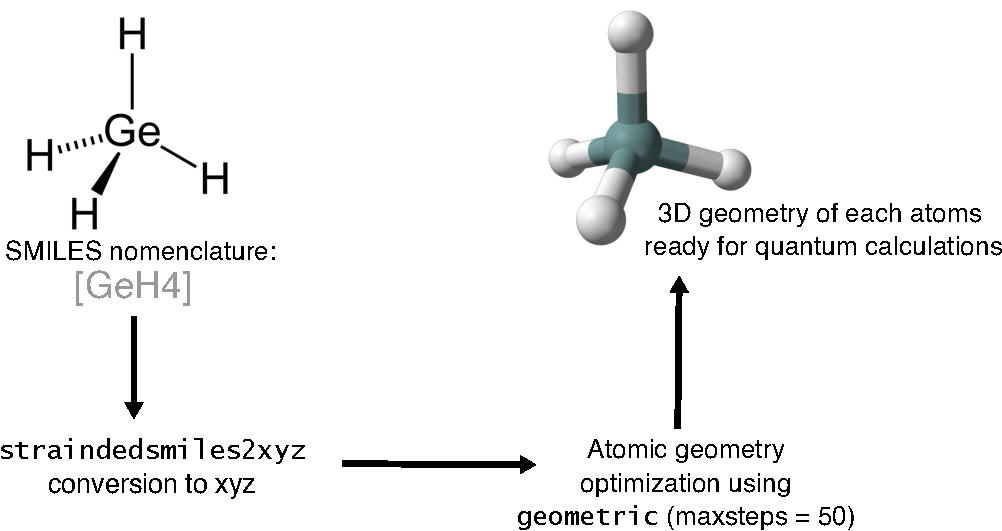
\includegraphics[width=\columnwidth]{mol_svg/path13.pdf}
    \caption{Overview of the molecular geometry pipeline for molecules without 3D conformer available. Germane \ch{GeH4} is used as an example.}
    \label{fig:sssss}
\end{figure}



\subsection{The BEB method for TICS calculation} 
The \textit{Binary Encounter Bethe} (BEB) method proposed by \textcite{kimBinaryencounterdipoleModelElectronimpact1994} as became the standard for theoritical TICS calculations, aswell as being suggested in papers about methods using TICS as parameters \parencites{gautier}. It was proposed as a much simplier model than the \textit{Binary Encounter Dipole} (BED) for ionisation cross-sections calculation. The BEB method estimates the cross-section of total ionisation using the electron energy of the Molecular Orbital (MO) and the kinetic energy of the electron whithin. In application, the BEB method can expressed as, for a distinct MO $i$:
\begin{align}
    \sigma_{i}(T) = \frac{S}{t+u+1} \left[\frac{\ln t}{2} \left(1-\frac{1}{t^2}\right)+1-\frac{1}{t}-\frac{\ln t}{t+1}\right] \label{eq:beb}
\end{align}
with $t=\frac{T}{B}$, $u=\frac{U}{B}$, where $T$ the ionisation particle energy and B and U are the  aforementioned MO electrons and kinetic energy, and S is expressed as:
\begin{align}
    S = 4\pi a_0^2N_i\left(\frac{R}{B}\right)^2 \label{eq:S}
\end{align}
with $a_0$ the Bohr radius (0.5292 $\AA$), $R$ the Rydberg constant (13.6 eV) and $N_i$ the number of electrons in the MO. For neutral stable species, N is always equal to 2. This, however, gives the cross section for only one MO. To get the total ionisation cross section, we need to sum all the $\sigma_i(T)$ of each MO, which gives us:
\begin{align}
    \sigma_{TICS}(T) = \sum^n_{i=1} \sigma_i(T)
\end{align}
Concerning $T$, this parameter is kept at relatively low energy. As it is, intermediates steps of the calculations, \textit{e.g} the $\sigma_i$, do not represents partial ionisation cross-section. \textcite{jesenekPartialIonisationCross2025} explains that and proposed a modified approach of the BEB method for such purposes. We considered 10$^3$ values in a logscale array with $T~\in~[10^1;10^5]$ eV.  

\subsection{Quantum chemistry parameters calculations}\label{sec:quantum}
As such, BEB calculations requires the MO electrons energies (B) as well as their kinetic energies (U) . While NIST database propose this parameter for several molecule\footnote{\url{https://physics.nist.gov/PhysRefData/Ionization/molTable.html}}, this is limited in terms of selection. One way is to calculate these parameter. To do that, PySCF quantum chemistry model \parencites{sunPythonbasedSimulationsChemistry2017}  was employed. Using the downloaded geometries, we can input them into the model and obtain the required paramaters. This model is based on the Self Consistent Field (SCF) method of quantum chemistry for the HF approach. The basis-set family used in this work is the Karlsruhe \verb+def2-TZVPPD+ basis-set -- valence triple-zeta with sets of polarization and diffuse functions \parencites{weigendBalancedBasisSets2005,rappoportPropertyoptimizedGaussianBasis2010}. Although a quadruple-zeta (QVZ) basis set could have been used, we used a triple-zeta (TVZ) basis set in this work for computational reasons. This type of basis, in particular the \verb|def2-TZVPP| basis, is proven to be reliable for HF modeling for a majority of the periodic table, from H up to Rn \parencites{hellwegDevelopmentNewAuxiliary2015,zhengMinimallyAugmentedKarlsruhe2011}. Several BEB-related papers use either the cross-correlated Dunning \textcite{dunningGaussianBasisSets1989} \verb|cc-| base \parencites{gachesAstrochemistryLowenergyElectron2024,kumarElectronIonizationCross2014} or Pople \parencites{krishnanSelfconsistentMolecularOrbital1980} gaussian \verb|6-311G| basis \parencites{aliElectronimpactTotalIonization1997, hwangNewModelElectronimpact1996, scottElectronImpactIonizationCross2005}. At our knowledge, this is the first use of a \verb|def2-| basis for TICS calculations. Only Restricted Hartree-Fock (RHF) calculations were performed, as all molecules are neutral and stable and thus have closed shell.

Regarding the energies output of the model, we first assume that $B$ is the absolute value of the lowest electron binding energy of the orbital, \textit{e.g} the first ionisation potential (IP) which satisfies the Koopmans theorem \parencites{koopmansUberZuordnungWellenfunktionen1934} $B = -\epsilon_i$, with $\epsilon_i$ the first ionisation energy of an orbital $i$. Whilst this is a good approach that is easy to implement and are directly obtained though the HF calculations, this does involve some simplifications as the orbitals are considered as "frozen", meaning that the other electrons do not react to the removal of ionized electron and that the post-ionization orbitals aren't be relaxed. This leads to overestimated first ionization potential for each orbitals \parencites{colonnaKoopmansCompliantFunctionalsPotentials2019, wangIonizaPotenJP102026,jesenekPartialIonisationCross2025,scottElectronImpactIonizationCross2005}. However, alternative approach such as outervalence Green’s function (OVGF; \cite{vonniessenComputationalMethodsOneparticle1984}), coupled cluster (CC, generally single-double-triple CCSDT; \cite{cizekCorrelationProblemAtomic1966}) require higher computational effiort. While some TICS-related papers use those approach \parencites{scottElectronImpactIonizationCross2005,gachesAstrochemistryLowenergyElectron2024}, the BEB method was historically built around HF method and $B$, as well as IP, were either experimental values or theoritical values. Furthermore, first ionization potential approach is widely used in other BEB-related papers \parencites{aliElectronimpactTotalIonization1997, hwangNewModelElectronimpact1996, gravesEfficientCalculationElectron2021} and do provide accurate results.
\textcite{gachesAstrochemistryLowenergyElectron2024} proposed a derived BEB method, namely dBEB, which takes IP values in account to scale BEB TICS as close as possible to experimental data by dampening the impact of high energies of orbitals. The $B$ parameter in relation \ref{eq:beb} and \ref{eq:S} can be expressed as :
\begin{align}
    B\prime = B\cdot\exp\left[-1\left(1-\frac{B}{IP}\right)\right]
\end{align}
One way to get accurate IP values are post-HF methods, as direct HF output IP may be too approximate \parencites{scottElectronImpactIonizationCross2005,wangGeometryOptimizationMade2016}. We already discussed of complex method such as CCSSD(T) before, but such implementation require large amount of computational power. A less demanding method is to use Density Functionnal Theory (DFT) to overcome the assumptions. We can use the $\Delta DFT$ method to calculate the first ionisation potential of an orbital, as, for a given orbital $i$ of an atom $N$  \parencites{wangFe3dOrbital2025}:
\begin{align}
    \Delta DFT = E_{i,N^+} - E_{i,N} = IP
\end{align}
with $E_{i,N^+}$ the energy of a OM of the cation state of the molecule and $E_{i,N}$ the MO energy of the neutral state. Calculation are done using the Coulomb-Attenuating Method (CAM) with the B3LYP functional \parencites{yanaiNewHybridExchange2004}. Compared to direct HF output, the $\Delta DFT$ showcase results much more closer to litterature values, as seen in table \ref{tab:zezeze} in the appendix, where comparison of our calculated IP with IP obtained though other means is made. As seen in this table, HF IP output values tend to be higher than post-HF values methods. Regarding kinetic energy $U$, this not a direct output of the model and it needs to be derived. As such, $U$ is calculated as:
\begin{align}
   U_i = \textrm{\bfseries Tr } \textrm{\bfseries C}_i^\textrm{ \bfseries T} \textrm{\bfseries T} \textrm{\bfseries C}_i
\end{align}
with $\textrm{\bfseries C}_i$ the MO coefficient matrix of the orbital $i$ in the Linear Combinaison of Atomic Orbital (LCAO)\footnote{For a given guess wave function $\phi_j(\textrm{\bfseries r})$: $\phi_j = C_{\mu j}\chi_\mu(\textrm{\bfseries r})$ with $C_{\mu j}$ the expansion coefficient and $\chi_\mu$ the atom centered Gaussian basis function.} formalism and $\textrm{ \bfseries T}$ the kinetic energy matrix that is composed by elements as
 \begin{align}
\textrm{\bfseries T}_{xy} = \langle \chi_x | -\frac{1}{2}\nabla^2 | \chi_y \rangle
\end{align}
% https://mattermodeling.stackexchange.com/questions/11014/computing-the-kinetic-energy-of-a-molecular-orbital
%https://doi.org/10.1039/b508541a celui là il est vener
%https://doi.org/10.1039/c4cp04286g
%https://link.springer.com/article/10.1007/s00214-010-0846-zsdsd sdsd
%https://pmc.ncbi.nlm.nih.gov/articles/PMC10208678/table/t4/

The BEB method, by itself, has limitations for heavy elements, with quantum number $n~>$ 2 or $Z~>$ 10 \parencites{gravesEfficientCalculationElectron2021,huoUseRelativisticEffective2000,aliIonizationCrossSections2008,scottElectronImpactIonizationCross2005}. The discrepancy arises because the BEB method uses, as shown in Eq.~\ref{eq:beb}, the kinetic energy of each molecular orbital as a variable. This is problematic for heavier elements, as inner electronic layers of this type have very high kinetic energies. However, ionisation should occur when the electron is far from the centre of the shell, i.e. when it is slower and thus has a lower kinetic energy. An overestimation of the kinetic energy leads to an underestimation of $\sigma_{\text{TICS}}$. The solution proposed by \textcite{huoUseRelativisticEffective2000}, and employed in several BEB-related studies on heavy elements \parencites{gravesEfficientCalculationElectron2021,dolgRelativisticPseudopotentialsTheir2012,scottElectronImpactIonizationCross2005}, is to use the effective core potential (ECP) method. An ECP limits the interaction of valence electrons with the core shell by replacing the latter with analytical functions that represents the interaction between the two. These functions appear as effective potential, while the valence electrons are described by pseudo-valence orbitals that do not penetrate the inner region of the nucleus. In a nut\textit{shell}, the ECP enables the removal of high kinetic energies of core electrons from the BEB sum, as core electrons do not intervene in electronic bonds, which would otherwise artificially minimalize $\sigma_{TICS}$.
The ECP method can be used in PySCF and, in order to include as many molecules as possible in the database, was implemented in this work. This, however, requires a different basis than the all-electrons Karlsruhe \verb+def2-+, because its related ECP basis only start at Rb ($Z~\geq$ 37) and thus don't work for lighter elements, \textit{e.g} $3p$ and $4p$ elements. The only basis that has an ECP basis that supports  these that is inherently available in PySCF and in the Basis Set Exchange database\footnote{\url{https://basissetexchange.org/}} \parencites{pritchardNewBasisSet2019} is the \verb|crenbl| basis set \parencites{hurleyInitioRelativisticEffective1986,fernandezpaciosInitioRelativisticEffective1985}. More modern basis are available on the open-source Pseudopotentiallibrary\footnote{\url{https://pseudopotentiallibrary.org/}}, as it provides Dunning derived basis combo for both $3p$ and $4p$ elements.  For Al, Si, P, S, Cl and Ar bearing molecules, we used the \verb|aug-cc-pVTZ| orbital basis along with its associated ECP basis proposed by \parencites{bennettNewGenerationEffective2018}, whereas for Ge, As, Se and Br bearing molecules we used the same orbital basis and the ECP basis proposed by \parencites{wangNewGenerationEffective2019}. The choices of those basis are also applied to post-HF method discussed earlier. The impact of ECP on TICS calculation is discussed in subsection \ref{sec:ecp}. Overall, the whole methodology employed in this work is summarized on figure \ref{azzada}

\begin{figure*}[!htb]
    \centering
\fbox{
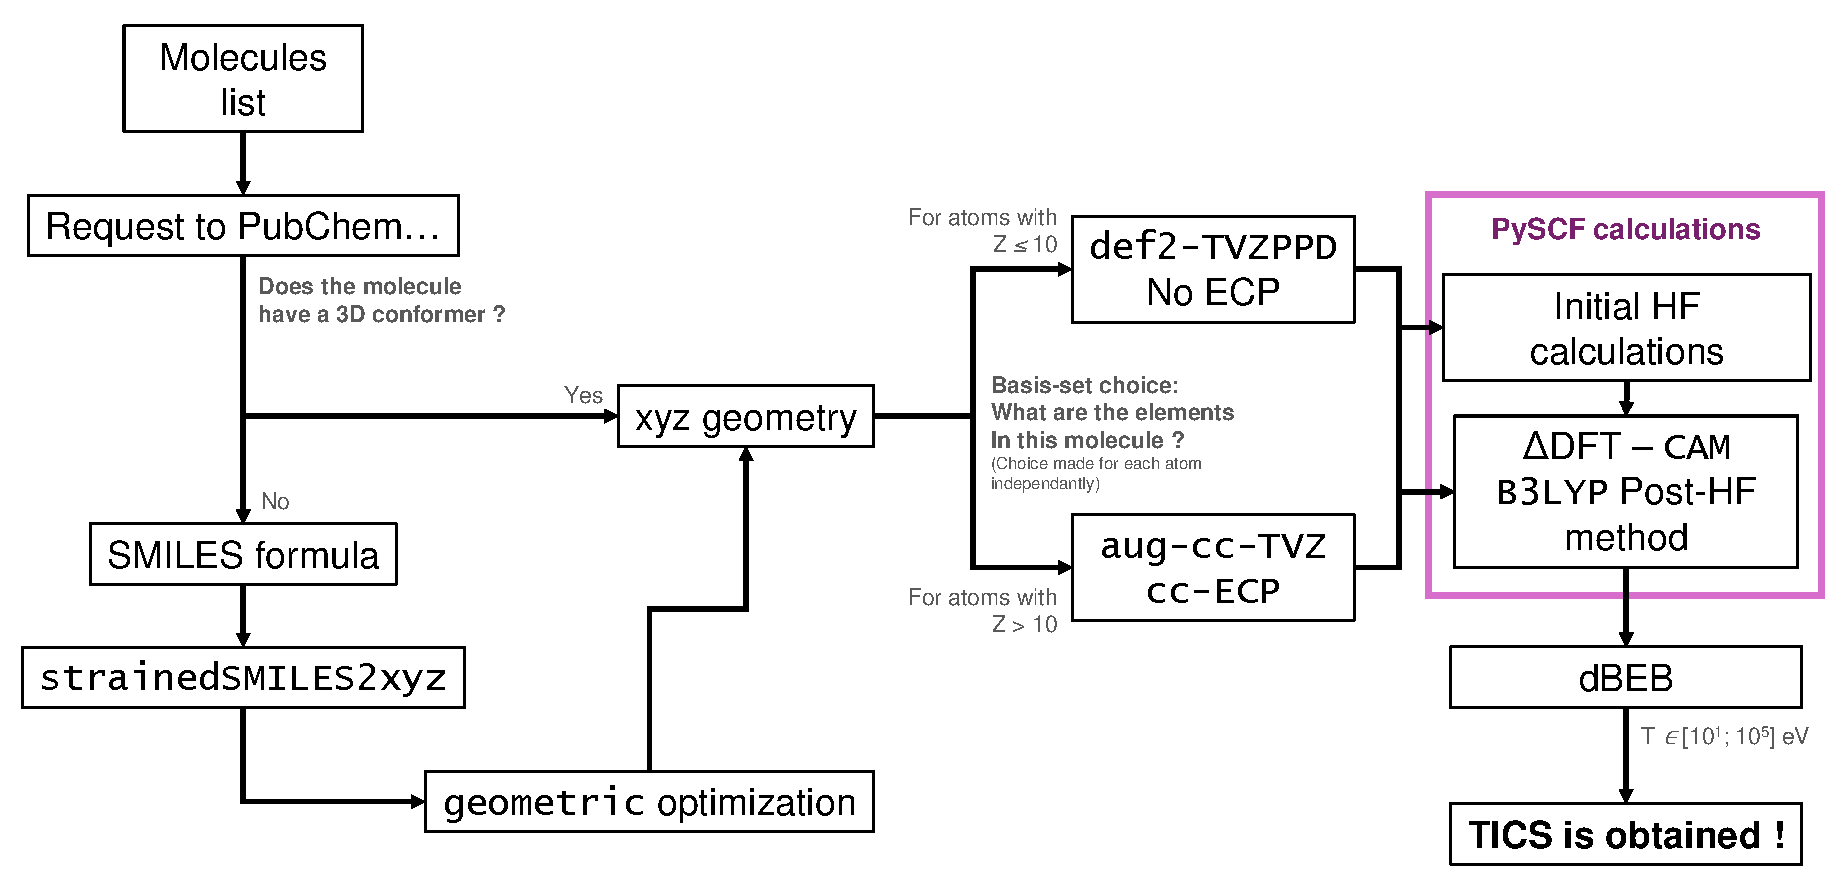
\includegraphics[width=1\linewidth]{figure/Présentation2.pdf}}
    \caption{Overview of the general workflow and methodology employed in this work.}
    \label{azzada}
\end{figure*}



\section{Results}
\subsection{Overview}
260 total ionisation cross section of unique molecules have been calculated, and up to 9 isomer for some formula such as \ch{C6H12}. The complete list is visible on table \ref{tab:fouzinzin}. On the database website, the user can find the TICS table of each molecule, along with a table with the calculated $B$ and $U$ values for each molecular orbital following the chosen basis aswell as the calculated IP. 

\begin{table}[ht!]
\centering
\caption{List of molecules present in the database. Superscript number indicates the number of isomers. Grey molecules indicates that no 3D conformer was available on PubChem and that the geometry was generated from SMILES structure.}
% sdsd
\label{tab:fouzinzin}
\setlength{\tabcolsep}{3pt}
\centering
\tiny
\begin{tabular}{@{}cccccccccccccc@{}}
\toprule
\multicolumn{14}{c}{Number of atoms}\\
\midrule
1 & 2 & 3 & 4 & 5 & 6 & 7 & 8 & 9 & 10 & 11 & 12 & 13 & $\geq 14$\\
\midrule
 & \ch{AlCl} & \ch{CHN}\textsuperscript{2} & \ch{\color{gray}AsH3} & \ch{C2H2O} & \ch{C2Cl4} & \ch{C2H3NO}\textsuperscript{2} & \ch{C2H4N2} & \ch{C2H5NO}\textsuperscript{2} & \ch{C2H5NO2} & \ch{C2H7NO} & \ch{C3H6O3} & \ch{C3H8O2}\textsuperscript{2} & \ch{C17H9N}\textsuperscript{3}\\
 & \ch{AlF} & \ch{CHP} & \ch{C2H2} & \ch{C2H2S} & \ch{C2H2O2} & \ch{C2H4O}\textsuperscript{3} & \ch{C2H4O2}\textsuperscript{4} & \ch{C2H6O}\textsuperscript{2} & \ch{C2H6O2}\textsuperscript{2} & \ch{C3H6O2}\textsuperscript{2} & \ch{C3H7NO} & \ch{C3H9N}\textsuperscript{3} & \ch{C16H10}\\
 & \ch{Br2} & \ch{CO2} & \ch{C2N2}\textsuperscript{2} & \ch{C2HNO} & \ch{C2H3Cl} & \ch{C2H4S}\textsuperscript{2} & \ch{C2H5N}\textsuperscript{2} & \ch{C2H6S}\textsuperscript{2} & \ch{C2H6OS} & \ch{C3H7N} & \ch{C3H8O}\textsuperscript{3} & \ch{C3H9P} & \ch{C14H10}\\
 & \ch{BrH} & \ch{COS} & \ch{CH2O} & \ch{C3HN}\textsuperscript{2} & \ch{C2H3N}\textsuperscript{3} & \ch{C3H2N2} & \ch{C2H6} & \ch{C3H3N3} & \ch{C2H7N}\textsuperscript{2} & \ch{C3H8} & \ch{C4H6O2}\textsuperscript{2} & \ch{C4H8O}\textsuperscript{2} & \ch{C11H12N2O2}\\
 & \ch{C2} & \ch{CS2} & \ch{CH2S} & \ch{CCl4} & \ch{C2H4} & \ch{C3H3N} & \ch{C3H3NO}\textsuperscript{3} & \ch{C3H4N2}\textsuperscript{2} & \ch{C3H5NO} & \ch{C4H6O} & \ch{C4H7N}\textsuperscript{3} & \ch{C4H8S} & \ch{C11H7N}\textsuperscript{2}\\
 & \ch{CO} & \ch{ClNO} & \ch{CHNO}\textsuperscript{3} & \ch{CF4} & \ch{C2HCl3} & \ch{C3H4}\textsuperscript{3} & \ch{C3H3NS} & \ch{C3H5N} & \ch{C3H6O}\textsuperscript{4} & \ch{C5H5N} & \ch{C4H8}\textsuperscript{5} & \ch{C5H8}\textsuperscript{5} & \ch{C10H8}\\
 & \ch{CS} & \ch{FNO} & \ch{CHNS}\textsuperscript{3} & \ch{CH2Cl2} & \ch{C3H2O}\textsuperscript{4} & \ch{C3N4} & \ch{C3H4O}\textsuperscript{2} & \ch{C3H6}\textsuperscript{2} & \ch{C4H4N2}\textsuperscript{2} & \ch{C5H6} & \ch{C6H6}\textsuperscript{3} & \ch{C7H5N} & \ch{C9H8}\\
 & \ch{Cl2} & \ch{H2O} & \ch{H2O2} & \ch{CH2F2} & \ch{C4H2} & \ch{C5HN} & \ch{C4H3N}\textsuperscript{3} & \ch{C4H4S} & \ch{C4H5N}\textsuperscript{2} &  & \ch{C6N6} &  & \ch{C8H10}\textsuperscript{3}\\
 & \ch{ClH} & \ch{H2S} & \ch{H2S2} & \ch{CH2N2}\textsuperscript{2} & \ch{C4N2} & \ch{CH4Si2} & \ch{C4H4} & \ch{C5H4}\textsuperscript{2} & \ch{C4H6}\textsuperscript{4} &  &  &  & \ch{C8H8}\\
 & \ch{F2} & \ch{H2Se} & \ch{H3N} & \ch{CH2O2} & \ch{CH2O3} & \ch{CH5N} & \ch{C6H2} &  &  &  &  &  & \ch{C7H8}\textsuperscript{2}\\
 & \ch{FH} & \ch{HNO} & \ch{H3P} & \ch{CH2S2} & \ch{CH3NO} & \ch{N2O5} & \ch{C6N2} &  &  &  &  &  & \ch{C6H10}\\
 & \ch{H2} & \ch{N2O} & \ch{HNO2} & \ch{CH3Br} & \ch{CH3NS} &  & \ch{CH3ClO2S} &  &  &  &  &  & \ch{C6H12}\textsuperscript{9}\\
 & \ch{N2} & \ch{O2S} & \ch{HNOS} & \ch{CH3Cl} & \ch{CH3NSi} &  & \ch{CH4N2O} &  &  &  &  &  & \ch{C6H14}\textsuperscript{4}\\
 & \ch{OSi} & \ch{O3} & \ch{O3S} & \ch{CH3F} & \ch{CH4O} &  & \ch{H6Si2} &  &  &  &  &  & \ch{C6N8}\\
 &  &  &  & \ch{CH3I} & \ch{CH4S} &  &  &  &  &  &  &  & \ch{C5H10}\textsuperscript{3}\\
 &  &  &  & \ch{CH3P} & \ch{H4N2} &  &  &  &  &  &  &  & \ch{C5H12}\\
 &  &  &  & \ch{CH4} & \ch{N2O4} &  &  &  &  &  &  &  & \ch{C5H8O}\\
 &  &  &  & \ch{CHCl3} &  &  &  &  &  &  &  &  & \ch{C4H10}\textsuperscript{2}\\
 &  &  &  & \ch{CHF3} &  &  &  &  &  &  &  &  & \ch{C4H10O}\textsuperscript{4}\\
 &  &  &  & \ch{\color{gray}GeH4} &  &  &  &  &  &  &  &  & \ch{C4H10S}\\
 &  &  &  & \ch{H3NO} &  &  &  &  &  &  &  &  & \ch{C4H8O2}\textsuperscript{3}\\
 &  &  &  & \ch{H4Si} &  &  &  &  &  &  &  &  & \ch{C3H8O3}\\
 &  &  &  &  &  &  &  &  &  &  &  &  & \ch{C3N12}\\
\bottomrule
\end{tabular}
\end{table}

\subsection{ECP impact on TICS calculation}\label{sec:ecp}
On table \ref{tab:ecp} we compared the mean $\Delta$ of TICS between ECP and non-ECP calculations for $3p$ and $4p$ elements bearing molecules.  We compared the results of the \verb|cc-ECP| basis aswell as with the \verb|crenbl| basis with the \verb|def2-| basis. The mean $\Delta$ percentage is calculated, for the peak region ($T \in [10^1; 10^3]$ eV), as:
\begin{align}
   \overline{\Delta\sigma_{TICS}} (\%)= \Bigl \langle \frac{\sigma_{TICS}^{\textrm{ECP}} - \sigma_{TICS}^{\textnormal{def2-}}}{\sigma_{TICS}^{\textnormal{ECP}}} \times 100 \Bigr \rangle
\end{align}
\begin{figure}[!htb]
    \centering
    \includegraphics[width=\linewidth]{/home//lilian.heydel/Codes/CASEI/ECP_Test/comparaison_3_bases.pdf}
    \caption{Comparison of TICS results for several molecule with and without ECP enabled}
    \label{fig:ecp}
\end{figure}
with $\sigma_{\textnormal{ECP}}$ the TICS calculated with either \verb|cc-ECP| or \verb|crenbl|.  Figure \ref{fig:ecp} shows this comparison for several molecules. 
As expected, and as proposed is \textcite{huoUseRelativisticEffective2000} as well as in other BEB-related studies on heavy elements \parencites{gravesEfficientCalculationElectron2021,dolgRelativisticPseudopotentialsTheir2012,scottElectronImpactIonizationCross2005}, the use of ECP basis leads to a higher TICS value. We can see on table \ref{tab:ecp} that the increase are ranging from roughly 10\% for $3d$ elements up to almost 30\% for $4d$ elements bearing molecules. The latter ones -especially- are the one where ECP really affect the whole calculus. For germanium and selenium bearing molecules ($4d$), as well as bromium bearing molecules ($3d$) 


The downside of the ECP method is that the removal of core electrons do impact high energy TICS. This can be seen on figure \ref{fig:ecp} where, for some molecules, the non-ECP curves overlaps the ECP curve. For mass-spectrometry however, the general of the electron is generally in the peak region.

The use of ECP with dBEB shouldn't be a problem as IP is linked to valence electrons and not core, so the mix between the two should work.
\begin{table}[H]
    \centering
    \caption{Mean $\Delta$ of TICS between ECP and non-ECP calculations for $3p$ and $4p$ elements bearing molecules.}
    \label{tab:ecp}
\begin{tabular}{@{}l S[table-format=2.1] S[table-format=2.1]@{}}
        \toprule
        & \multicolumn{2}{c}{$\overline{\Delta\sigma}$ (\%)} \\
        \cmidrule(l){2-3}
        Molecule & {cc-ECP} & {CRENBL} \\
        \midrule
        \ch{H3P} & 13.996 & 14.568 \\ 
        \ch{H4Si} & 6.505 & 7.311 \\ 
        \ch{H6Si2} & 9.242 & 9.283 \\ 
        \ch{GeH4} & 27.548 & 32.212 \\ 
        \ch{H2Se} & 27.384 & 31.159 \\ 
        \ch{H2S} & 18.474 & 16.958 \\ 
        \ch{Ch3Br} & 20.059 & 22.418 \\ 
        \ch{BrH} & 24.582 & 27.666 \\ 
        \ch{Br2} & 26.276 & 26.496 \\ 
        \ch{Cs} & 11.996 & 0.948 \\ 
        \ch{Cl2O} & 18.123 & 12.592 \\ 
        \ch{OSi} & 5.703 & 6.007 \\ 
        \ch{CSi} & 7.079 & 7.372 \\ 
        \ch{Ch4Si2} & 5.093 & 7.995 \\ 
        \ch{Ch3NSi} & 2.749 & 3.753 \\ 
        \ch{C4H10S} & 9.545 & 9.718 \\ \bottomrule
    \end{tabular}
\end{table}


% https://pubs.aip.org/aip/jcp/article-abstract/160/9/094310/3268619/Electron-impact-partial-ionization-cross-sections?redirectedFrom=fulltext
% https://arxiv.org/pdf/2312.13001v3
% jpp mettre trop de figures de comparaison, pourquoi pas faire le delta avec de la littérature et prendre la moyenne ?


%https://www.ifi.unicamp.br/~maplima/artigos/ref120.pdf
%%% The values of the binding energies B and the kinetic energies U needed in the calculation
%of σBEB(T ) for these isomers were computed using the package GAMESS [21] in a RHF
%calculation with a 6-311++G(2d) basis set

%https://sci-hub.fr/10.1088/0022-3700/18/16/019


\begin{figure*}[p]
    \centering
    \includegraphics[width=1\linewidth]{/home/lilian.heydel/Codes/CASEI/plots_litt/plot1.pdf}
    \caption{Calculted TICS for several hydrocarbons. In those plots, $\sigma_{TICS}$ as been cropped at $10^{-8}$. Scatter plot mean experimental data and line plot mean theoritical data. Those data come from \textcite{rappTotalCrossSections1965,jiaoElectronImpactIonization2007,chathamTotalPartialElectron1984,aliElectronimpactTotalIonization1997, }. The references marked with an * where obtained through lxcat.com database \parencites{lxcat,carboneDataNeedsModeling2021,pitchfordLXCatOpenAccessWebBased2017,pancheshnyiLXCatProjectElectron2012}. Those references include }.
    \label{fig:hydro}
\end{figure*}
% sqdsdsdssds
\begin{figure*}[p]
    \centering
    \includegraphics[width=1\linewidth]{/home/lilian.heydel/Codes/CASEI/plots_litt/plot2.pdf}
    \caption{Calculted TICS for several organic and non-organic molecules. In those plots, $\sigma_{TICS}$ as been cropped at $10^{-8}$. Scatter plot mean experimental data and line plot mean theoritical data. Those data come from \textcite{rappTotalCrossSections1965,jiaoElectronImpactIonization2007,chathamTotalPartialElectron1984,aliElectronimpactTotalIonization1997,kumarElectronIonizationCross2014}. The references marked with an * where obtained through lxcat.com database. Those references include }  
      \label{fig:orga}
\end{figure*}

\section{Discussion}
\subsection{Comparison with literature}
In order to validate our results, we compared our calculated TICS with several experimental and theoretical data from the literature. Our main benchmark are the values presented in \textcite{gachesAstrochemistryLowenergyElectron2024}, as they had done an impressive work of gathering data for a large amount of species.
\subsubsection{Hydrocarbons}
As pointed out by \textcite{hwangNewModelElectronimpact1996}, the BEB method is very efficient for hydrocarbons BEB calculations. As seen on figure \ref{fig:hydro}, our curves fit well to either experimental nor theoritical values. As intented, for some molecules, such as methane \ch{CH4} or acetylene \ch{C2H2}, experimental $B$ values tend to be smaller than theoritical/computed $B$ values \parencites{aliElectronimpactTotalIonization1997,hwangNewModelElectronimpact1996}. As such, the cross section obtained through experimental $B$ values tend to be higher,$ \approx$10-15\% at the cross section peak. This is mitigated either by the errorbar of experimental values (that are generally around 20\%; \cite{jiaoElectronImpactIonization2007}) or by the dampening of the dBEB method. Regardless, the data obtained though our pipeline do match litterature data for hydrocarbons.\\
Aromaticity shouldn't, in theory, impact BEB calculations. As such, we modelised a few polycyclic aromatic hydrocarbons (HAPs) in the database. Like \textcite{gachesAstrochemistryLowenergyElectron2024}, from the most simple benzene \ch{C6H6} to pyrene \ch{C16H10}. The biggest present in \textcite{gachesAstrochemistryLowenergyElectron2024} is anthracene \ch{C14H10}. In that case our data have pretty good relation with litterature data.
The historical papers of the beb method, \textit{e.g} \textcite{hwangNewModelElectronimpact1996,kimBinaryencounterdipoleModelElectronimpact1994}, show that limit of the BEB method regard the electronic atom size rather than the molecule size (see subsubsection \ref{subsub:heavy}). That is why we also got a good agreement with more complex HAPs like pyrene. In theory, one would be able to modelise 
% The BEB ionization cross section is sensitive to the vertical ionization energy of the molecule, that is, the ionization threshold. 

\subsubsection{Nitrogen bearing molecules}
Ca fonctionne pour celle de la litt mais en plus nous on a des trucs de zinzin fou genre le proprionytil ou les trucs en 3D

\subsubsection{Oxygen bearing molecules}
Ca marche

\subsubsection{Sulfur and phosphorus bearing molecules}
Ca marche et ca marche meme "mieux" que \textcite{gachesAstrochemistryLowenergyElectron2024} pcq on a l'ECP. Pour les molécules concernées ca colle niquel. Par contre H2S aucune idée de pourquoi c'est décalé un peu
Benef pour PH3, y'a 0 papier expérimentaux mais on colle bien au indiens

\subsubsection{Heavy elements bearing molecules}\label{subsub:heavy}

Le germane et le selane, jsp quoi dire d'autre ? Trouver data sur le sujet

% \begin{figure}[!htb]
%     \centering
%     \includegraphics[width=1\linewidth]{/home/lilian.heydel/Codes/CASEI/plots_litt/plot3.pdf}
%     \caption{Comparison for rare gases}
%     % Pas sûr que cette figure soit judicieuse
%     \label{fig:placeholder}
% \end{figure}

% \lipsum
% Y'a un truc cool que je pourrais faire c'est essayer de comparer les molécules du butane avec des extensions genre C4H10O ou S
% mais y'a pas de papiers là dessus
% mais en gros montrer que l'isomérie a en réalité assez peu d'impact sur le sigma (j'ai vu ca avec C6H12 par ex) mais qu'un hétéroatome qui se branche dessus peut faire des choses
% \section{Limit of this work} Limite dans les discussions

\subsection{Impact of isomery on TICS calculation}
A few papers shown that isomery should affect TICS. 

\begin{figure}[!htb]
    \centering
    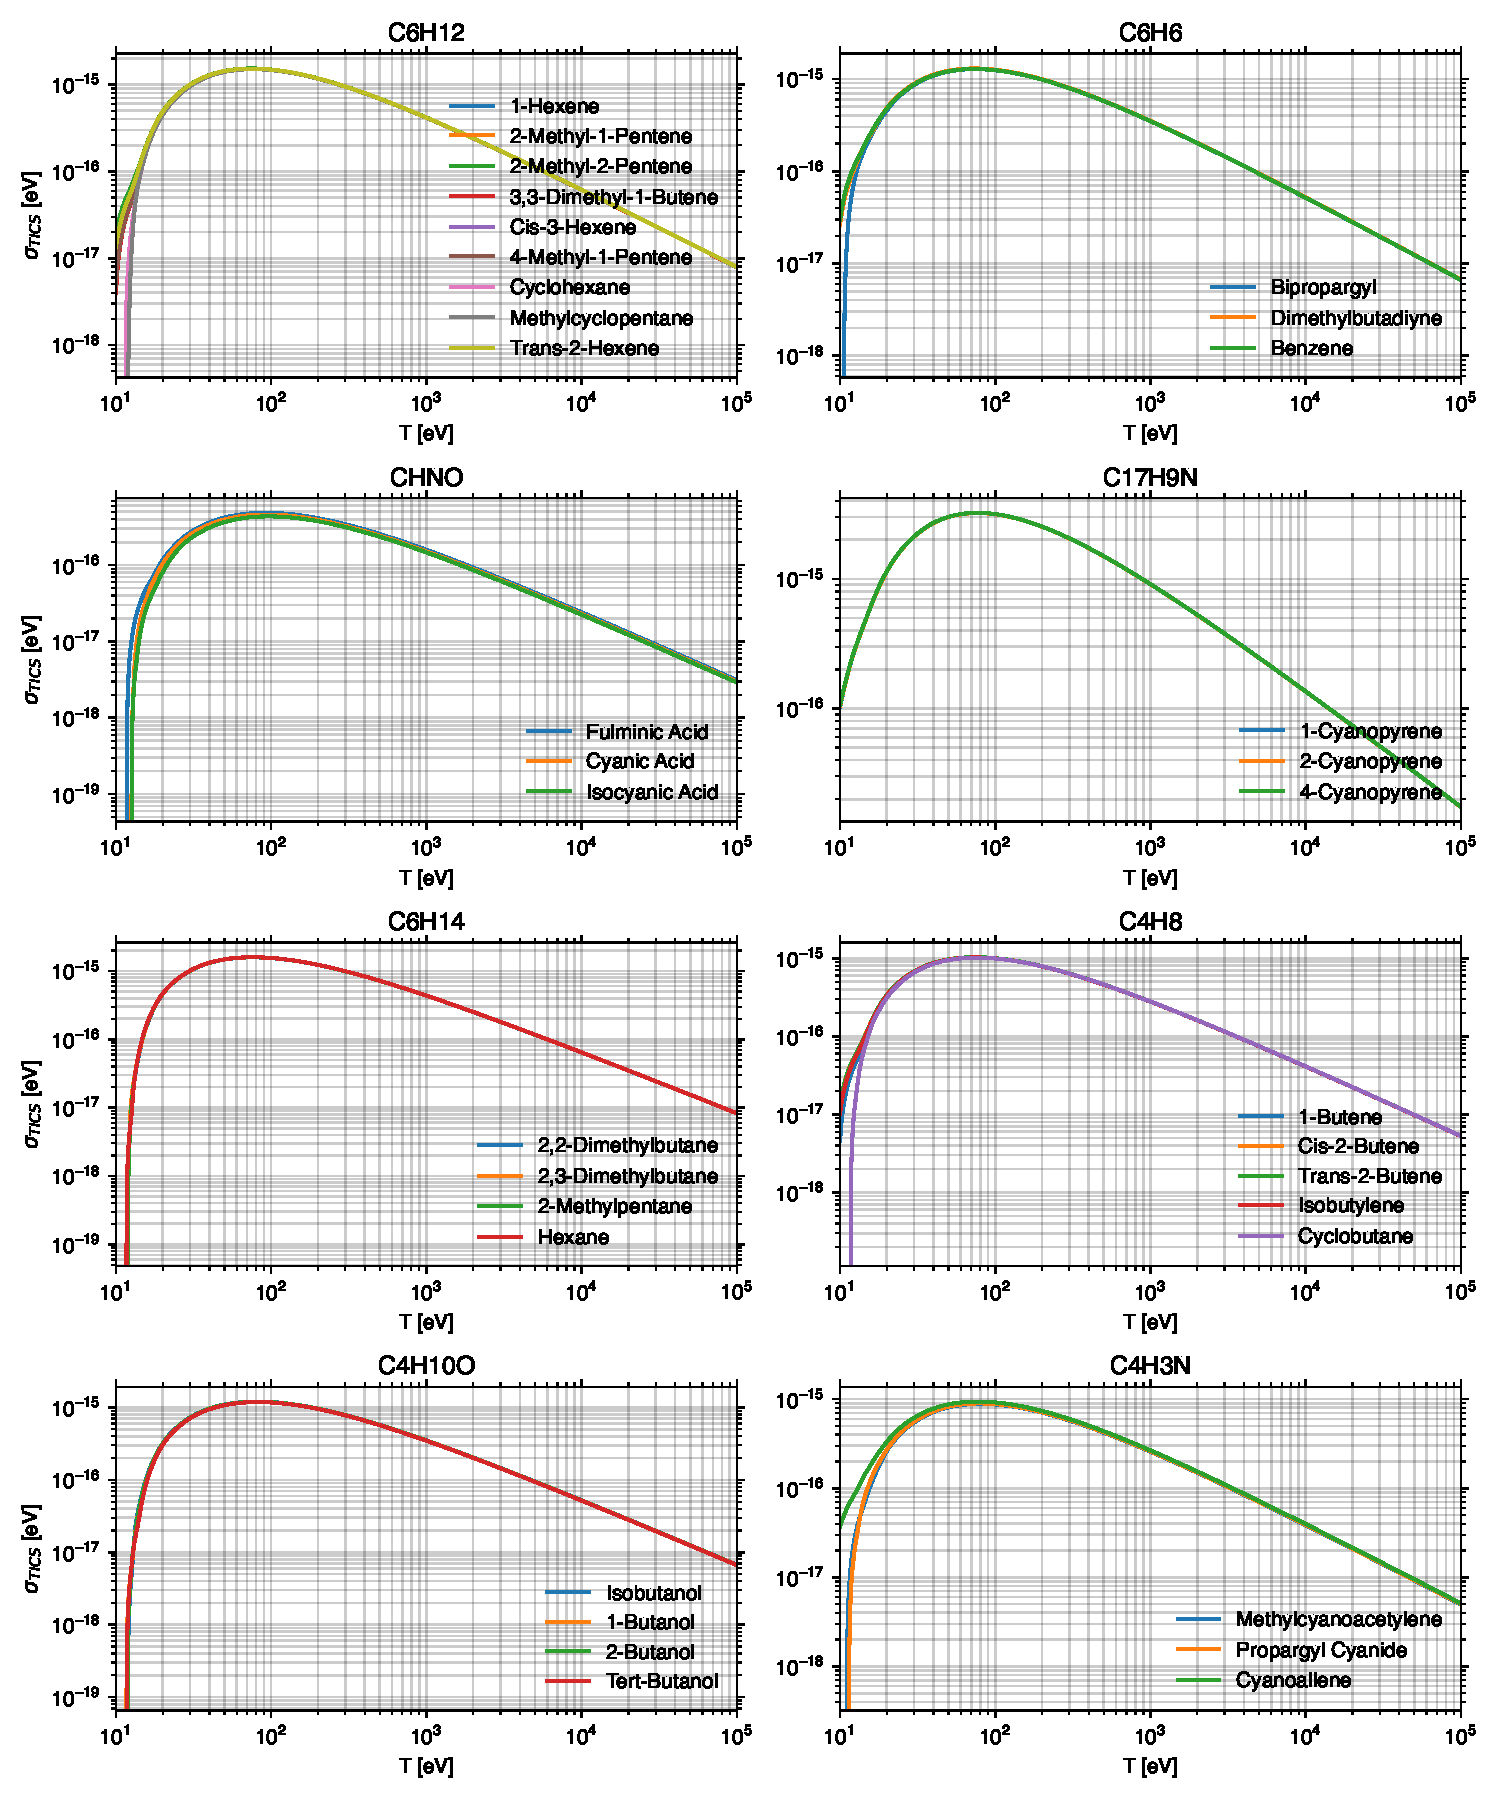
\includegraphics[width=\textwidth]{figure/compare_iso.pdf}
    \caption{dfbsdkfgk}
\end{figure}


\subsection{Applications to mass spectrometry}
Ici trouver une idée

\section{Conclusion}
In this paper we presented a computational pipeline for calculating theoritical total ionisation cross section of 260 neutral molecules.

Multiple outlook could be imaginated:
\begin{itemize}
    \item Adapt the pipeline for radicals (\textit{i.e} molecules with spin $\neq$ 0) and ions; This would require to do calculation using an Unrestricted Hatree-Fock (UHF) approach;
    \item Adapt and create a custom \verb|def2-| ECP basis for $3d$ and $4p$ elements in order to homogenize the database as much as possible protocol-wise;
    \item CCSD(T) calculation would enable better IP values for dBEB calculations.
\end{itemize}
%https://chemrxiv.org/doi/pdf/10.26434/chemrxiv-2021-hb50g-v2#5#12#5

% \section{References}
% The journal uses the American Psychological Association (APA) 7th edition style for references and citations. References can be cited textually in sentences, such as~\textcite{becker2015phd}, \textcite{Rudolph2020}, \textcite{bagnasco2017nirspec}, and \textcite{Breuer2015}. References can also be cited parenthetically~\parencites{dressler2006nasa,Neukumetal2001a,Wieczorek2022-preprint,SJOGRENdataset}. Each reference must contain a persistent identifier (such as a DOI) when one is available.

\section*{Acknowledgements}
Specify contributions that require acknowledgment but that do not warrant authorship. This may include acknowledgments of technical assistance, materials, or financial support. When persons are mentioned in the acknowledgments, the corresponding author should request their permission to appear in the text.

\section*{Open science declarations}

\noindent\textbf{Author contributions.} List here the details of each of the author's contributions to the work using the Contributor Role Taxonomy (CRediT, \href{https://credit.niso.org/}{https://credit.niso.org/}). These roles include: Conceptualization, Data curation, Formal analysis, Funding acquisition, Investigation, Methodology, Project administration, Resources, Software, Supervision, Validation, Visualization, Writing (original draft), and Writing (review \& editing). Only those roles that are appropriate should be specified. These roles are summarized in the journal's authorship policies: \href{https://planetary-research.org/authorship}{https://planetary-research.org/authorship}.

\noindent\textbf{Code availability.} Numerical codes must both be findable and accessible according to FAIR principles (\href{https://www.go-fair.org/fair-principles/}{https://www.go-fair.org/fair-principles/}). Findable means that the code can be located using a persistent identifier, such as a software heritage identifier SWHID, an astrophysics source code library identifier ASCL, or a DOI. The conditions under which the code and software used in a manuscript can be accessed must be described either on the landing page of the code or in the code archive. If the code is restricted and requires credentials to be accessed, the exact conditions under which the credentials can be obtained should be provided. For further information, see the journal's Open Science policies: \href{https://planetary-research.org/open-science}{https://planetary-research.org/open-science}.

\noindent\textbf{Data availability.} Any data that were used or generated as part of the study and that are not found in the manuscript and supplement must be uploaded to a public data repository before the article is accepted for publication. The datasets and any accompanying metadata and documentation should be made available to the reviewers during the peer-review process. For further information, see the journal's Open Science policies: \href{https://planetary-research.org/open-science}{https://planetary-research.org/open-science}.

\noindent\textbf{Funding.} All sources of funding for the work must be disclosed. For work funded by a research agency, the following information should be provided: The name of the funding agency, the name of the funding program, the title of the funded project, and the grant number or funding reference.

\noindent\textbf{Competing interests.} All manuscripts must declare any real or perceived conflicts of interest. Competing interests may include both financial and non-financial interests such as past or present employment, consulting activity, financing, intellectual property, ownership of financial assets, or advisory roles. In the case where there are no competing interests, one can use the statement: The authors declare that they have no known competing financial interests or personal relationships that could have appeared to influence the work reported in this paper.

% ------ Appendix ------------------------------------------------------------
% Letters do not have appendices
\IfStrEq{\articletype}{LETTER}{}{
\appendix
\counterwithin{figure}{section}
\renewcommand{\thefigure}{\thesection\arabic{figure}}
\counterwithin{table}{section}
\renewcommand{\thetable}{\thesection\arabic{table}}
\counterwithin{equation}{section}
\renewcommand{\theequation}{\thesection\arabic{equation}}

\section{Optimization of PubChem geometries}\label{app:geom}
To see if pubchem geometries require optmization, we chose several molecules
\section{Energy of first ionisation IP}
\begin{table}[!ht]
    \centering
    % \small
    \caption{Comparison of the energy of the ionization potential between this work ($\Delta$)DFT  and \textcite{gachesAstrochemistryLowenergyElectron2024} CCSD(T) and CAM-B3LYP calculations for first ionization potential IP.}
    \label{tab:zezeze}
    \begin{tabular}{llll}\toprule
        Molecule & $\Delta$DFT & \textcite{gachesAstrochemistryLowenergyElectron2024} (CCSD(T)) & \textcite{gachesAstrochemistryLowenergyElectron2024} (DFT) \\ \midrule
        \ch{CO  }&14,84 & 14,13 & 14,24 \\ 
        \ch{H2  }&16,23 & 16,45 & ~ \\ 
        \ch{H2S }& 10,45 & 10,52 & 10,43 \\ 
        \ch{H2O } &13,87 & 12,8 & 12,69 \\ 
        \ch{O3 } & 13,26 & 13,02 & 12,77 \\ 
        \ch{C2H2 }& 13,48 & 11,54 & 11,28 \\ 
        \ch{C2N2 }& 13,48 & 14,74 & 13,25 \\ 
        \ch{C3H2O} & 11,59 & ~ & 10,59 \\ 
        \ch{CH2O }& 12,15 & 11,04 & 10,88 \\ 
        \ch{CH2S }& 9,61 & 9,5 & 9,3 \\ 
        \ch{NH3 }& 11,73 & 11,04 & 10,22 \\ 
        \ch{CH4 }& 14,80 & ~ & 12,72 \\ 
        \ch{C2H4 }& 10,25 & ~ & 10,4 \\ 
        \ch{N2H4 }& 10,46 & ~ & 6,82 \\ 
        \ch{C4N2 }& 12,08 & ~ & 11,67 \\ 
        \ch{c-H2C3O} & 10,54 & ~ & 9,54 \\ 
        \ch{CH3NS} & 9,04 & ~ & 9,45 \\ 
        \ch{C4H2 }& 10,14 & ~ & 9,96 \\ 
        \ch{C2H6 }& 13,19 & ~ & 11,59 \\ 
        \ch{C6N2 }& 11,25 & ~ & 10,69 \\ 
        \ch{C4H4 }& 9,39 & ~ & 9,32 \\ 
        \ch{C5H4 }& 9,64 & ~ & 10,03 \\ 
        \ch{C3H8 }& 12,74 & ~ & 10,99 \\ 
        \ch{C4H10} & 12,28 & ~ & 10,89 \\ 
        \ch{c-C6H6} & 9,16 & ~ & 9,17 \\ 
        \ch{C14H10} & 6,74 & ~ & 7,21 \\ 
        \ch{C5H12} & 11,95 & ~ & 10,76 \\ 
        \ch{C6H14} & 11,69 & ~ & 10,77 \\ \bottomrule
    \end{tabular}
\end{table}


% end appendices
}

% ------ Methods section for LETTERS ----------------------
\IfStrEq{\articletype}{LETTER}{
\section*{Methods}
The Methods section is an optional section that is used only for the letter format. The methods section must be less than 3000 words in length and contain no tables or figures. The methods section is placed after the Open Science Declarations section.

% End methods section
}

% ------ Bibliography -------------------------------------
\printbibliography

% ------ License ------------------------------------------
% If you intend to distribute this manuscript, consider
% adding a CC-BY license by uncommenting the following
% line
% \license{}

\end{document}
